\documentclass[12pt,a4paper,]{article}
\usepackage{lmodern}
\usepackage{amssymb,amsmath}
\usepackage{ifxetex,ifluatex}
\usepackage{fixltx2e} % provides \textsubscript
\ifnum 0\ifxetex 1\fi\ifluatex 1\fi=0 % if pdftex
  \usepackage[T1]{fontenc}
  \usepackage[utf8]{inputenc}
\else % if luatex or xelatex
  \ifxetex
    \usepackage{mathspec}
  \else
    \usepackage{fontspec}
  \fi
  \defaultfontfeatures{Mapping=tex-text}
    \setmainfont[]{Tinos}
\fi
% use upquote if available, for straight quotes in verbatim environments
\IfFileExists{upquote.sty}{\usepackage{upquote}}{}
% use microtype if available
\IfFileExists{microtype.sty}{%
\usepackage{microtype}
\UseMicrotypeSet[protrusion]{basicmath} % disable protrusion for tt fonts
}{}
\usepackage[unicode=true]{hyperref}
\hypersetup{
            pdftitle={Open Science in phonetics and phonology},
            pdfauthor={Stefano Coretta},
            pdfborder={0 0 0},
            breaklinks=true}
%\urlstyle{same}  % don't use monospace font for urls
\usepackage{natbib}
\bibliographystyle{unified}
\usepackage{graphicx,grffile}
\makeatletter
\def\maxwidth{\ifdim\Gin@nat@width>\linewidth\linewidth\else\Gin@nat@width\fi}
\def\maxheight{\ifdim\Gin@nat@height>\textheight\textheight\else\Gin@nat@height\fi}
\makeatother
% Scale images if necessary, so that they will not overflow the page
% margins by default, and it is still possible to overwrite the defaults
% using explicit options in \includegraphics[width, height, ...]{}
\setkeys{Gin}{width=\maxwidth,height=\maxheight,keepaspectratio}
\setlength{\emergencystretch}{3em}  % prevent overfull lines
\providecommand{\tightlist}{%
  \setlength{\itemsep}{0pt}\setlength{\parskip}{0pt}}
\setcounter{secnumdepth}{5}
% Redefines (sub)paragraphs to behave more like sections
\ifx\paragraph\undefined\else
\let\oldparagraph\paragraph
\renewcommand{\paragraph}[1]{\oldparagraph{#1}\mbox{}}
\fi
\ifx\subparagraph\undefined\else
\let\oldsubparagraph\subparagraph
\renewcommand{\subparagraph}[1]{\oldsubparagraph{#1}\mbox{}}
\fi

% set default figure placement to htbp
%\makeatletter
%\def\fps@figure{htbp}
%\makeatother

\let\tnote\relax
\usepackage{cleveref}
\usepackage{ctable}
\usepackage{enumerate}
\usepackage{lineno}
\linenumbers

\title{Open Science in phonetics and
phonology\footnote{This preprint is a standalone version of a chapter from Stefano Coretta's PhD dissertation (Coretta, Stefano. 2020. Vowel duration and consonant voicing: A production study. University of Manchester dissertation.). Please use the OSF preprint DOI when citing.}}
\author{Stefano Coretta}
\date{22/01/2020}

\usepackage[absolute]{textpos}

\begin{document}
\maketitle

\hypertarget{introduction}{%
\section{Introduction}\label{introduction}}

Open Science is a movement that stresses the importance of a more honest
and transparent scientific attitude by promoting a series of research
principles and by warning from common, although not necessarily
intentional, questionable practices and misconceptions. The term Open
Science as a whole refers to the fundamental concepts of `openness,
transparency, rigour, reproducibility, replicability, and accumulation
of knowledge' \citep[3]{cruwell2018}. The goodness of the latter depends
in great part on the reproducibility and replicability of the studies
that contribute to knowledge accumulation. While reproducibility and
replicability are generally used interchangeably, they refer to two
different ideas. A study is \emph{replicable} when researchers can
independently run the study on new subjects/data and obtain the same
results (in brief, same analysis, different data/researchers). The
\emph{reproducibility} of a study is, instead, related to the ability of
independent researchers to run the original analysis on the original
data and obtain the same results as those presented by the original
authors, pending enough information on the analysis procedures is given
(in brief, same analysis, same data).

A sense of need for Open Science, now increasingly spreading to
different disciplines and enterprises, arose primarily from the ongoing
so-called `replication crisis' \citep{pashler2012, schooler2014}, which
has attracted the most attention within the circles of medical and
psychological sciences. Recent attempts to replicate results from
high-impact studies in psychology have demonstrated an alarmingly high
rate of failure to replicate. For example, in a replication attempt of
100 psychology studies, only 39\% of the original results were rated by
annotators as successfully replicated
\citep{open-science-collaboration2015}. Failure to replicate previous
results have been claimed to be a consequence of low statistical power
\citep{button2013}, and of so-called questionable research and
measurement practices \citep{simmons2011, morin2015, flake2019}. The
following sections discuss these problems in turn.

\hypertarget{with-great-power-comes-great-replicability}{%
\section{``With great power comes great
replicability''}\label{with-great-power-comes-great-replicability}}

One of the issues that can affect statistical analysis is related to
errors in rejecting the null
hypothesis.\footnote{The quote in the title is from a 2016 twitter status by Nathan C. Hall (\url{https://twitter.com/prof_nch/status/790744443313852417?s=20}).}
A researcher could falsely reject the null hypothesis when in fact is
correct (Type I errors, an effect is found when there is none), or they
could falsely fail to reject the null hypothesis when in fact it should
have been (Type II errors, an effect is not found when there is one).
Type I and Type II errors do occur and cannot be totally prevented.
Rather, the aim is to keep their rate of occurrence as low as possible.
The generally accepted rates of Type I and Type II errors are 0.05 and
0.2 respectively (usually referred to as the \(\alpha\) and \(\beta\)
levels). This means that, in a series of imaginary multiple replications
of a study, 5\% of the times the null hypothesis will be falsely
rejected, and 20\% of the times will falsely be not rejected. A concept
closely related to Type II errors is statistical power, which is the
probability of correctly rejecting the null hypothesis when it is false
(calculated as \(B = 1 - \beta\)). In other words, power is the
probability of detecting an effect equal or greater than a specified
effect size. Given the standard \(\beta = 0.2\), an accepted (minimum)
power threshold is 80\% (which means that an effect equal or greater
than a chosen size will be detected 80\% of the times).

Two other types of statistical errors are the Type S (sign) and Type M
(magnitude) errors \citep{gelman2000, gelman2014}. Type S errors refer
to the probability of the estimated effect having the wrong sign (for
example, finding a positive effect when in reality the effect is
negative), while Type M errors correspond to the exaggeration ratio (the
ratio between the estimated and the real effect). When the statistical
power of a study is low (below 50\%), \citet{gelman2014} show that the
exaggeration ratio (Type M error) is particularly high (from 2.5 up to
10 times the true effect size). Type S errors (wrong sign) are more
common at lower power levels (below 10\%), although these can easily
arise due to small sample sizes and high variance.

Several researchers have shown that the average statistical power of
studies in different disciplines is very low (35\% or below) and that
the last 50 years did not witness an improvement. \citet{bakker2012}
show that the median statistical power in psychology is 35\%, while
\citet{button2013} reports a median of 21\% obtained from 48
neuroscience meta-analyses. In \citet{dumas-mallet2017}, half of the
surveyed biomedical studies (N = 660) have power below 20\%, while the
median ranges between 9\% and 30\% depending on the subfield.
\citet{rossi1990} and \citet{marszalek2011} show that from the 70s to
date there hasn't been an increase in power and sample sizes.
\citet{tressoldi2015} also find that only 2.9\% of 853 studies in
psychology report a prospective power analysis for sample size
determination, i.e.~the estimation of the smallest sample size necessary
to obtain a certain power level before the experiment is run. In sum,
low statistical power (well below the recommended 80\% threshold) seems
to be the norm.

\hypertarget{the-dark-side-of-research}{%
\section{The dark side of research}\label{the-dark-side-of-research}}

Questionable research and measurement practices are practices that
negatively affect the scientific enterprise, but that are employed (most
of the time unintentionally) by a surprisingly high number of
researchers \citep{john2012}. \citet{silberzahn2018} asked 29 teams (61
analysts) to answer the same research question given the same data set,
and showed that data analysis can be highly subjective. A total of 21
unique combinations of predictors were used across the 29 teams, leading
to diverging results (20 teams obtained a significant result, while 9
did not). At various stages of the study timeline, a researcher can
exploit the so-called `researchers' degrees of freedom' to obtain a
significant result \citep{simmons2011}. The researchers' degrees of
freedom create a `garden of forking paths' \citep{gelman2013}, that the
researcher can explore until the results are satisfactory (i.e., they
lead to high-impact or expected findings).

\emph{P}-hacking is a general term that refers to the process of
choosing and reporting those analyses that change a non-significant
\emph{p}-value to a significant one
\citep{simmons2011, wagenmakers2007, motulsky2014}. \emph{P}-hacking can
be achieved by several means, for example by trying different dependent
variables, including and/or excluding predictors, selective
inclusion/exclusion of subjects and observations, or sequential testing
(collecting data until the results are significant). Another common
practice is to back-engineer a hypothesis after obtaining unexpected
results, also known as Hypothesising After the Results are Known
(HARKing, \citealt{kerr1998}). \citet{lieber2009} warns against `double
dipping', or the use of the same data to generate a hypothesis and test
it. \citet{morin2015} and \citet{flake2019} more specifically discuss
questionable practices related to how research variables are measured
and operationalised. The literature reviewed in \citet{flake2019}
suggests that a very high percentage of published papers contains
measures that are created on the fly but lack any reference to
reliability tests. Researchers have also been found to manipulate
validated scales to obtain desired results.

Cognitive biases and statistical misconceptions can also have a negative
impact on research conduct. \citet{wagenmakers2012} discuss the effects
of cognitive biases like the confirmation bias (the tendency to look for
facts and interpretations that confirm one's prior conviction,
\citealt{nickerson1998}) and the hindsight bias (the tendency to find an
event less surprising after it has occurred, \citealt{roese2012}).
\citet{greenland2017} defines further common distortions pertaining to
methodological approaches, like statistical reification (interpreting
statistical results as reflections of an actual physical reality).
Finally, \citet{wagenmakers2007} and \citet{motulsky2014} examine
mistaken beliefs about the meaning of \emph{p}-values and statistical
significance (like interpreting \emph{p}-values as an index to
statistical evidence or the idea that \emph{p}-values inform us about
the likelihood of the null-hypothesis given the data).

A bias in the observed effects can also arise at the stage of
publication. A publication bias has been observed in that significant
and novel results are generally favoured over null results or
replications
\citep{easterbrook1991, ioannidis2005, song2010, kicinski2013, nissen2016}.
\citet{rosenthal1979} called the bias agains publishing null results the
`file drawer' problem. Studies that don't lead to a significant result
are stored in a metaphorical file drawer and forgotten. This practice
not only can bias meta-analytical effect sizes, but also allows for
waste of resources when studies with undisclosed null results are
repeatedly performed. The questionable research and measurement
practices described above, together with publication bias, conspire to
unduly increase confidence in our research outcomes. A final exculpatory
note is due, though, in that these practices are not necessarily
intentional or fraudulent, and in some cases lie within a `grey area' of
accepted standard procedures.

\hypertarget{where-we-stand-and-where-we-are-heading}{%
\section{Where we stand and where we are
heading}\label{where-we-stand-and-where-we-are-heading}}

Given the similarities in methods between the psychological sciences and
phonetics/phonology, it is reasonable to assume that the situation does
not fare better in the latter. As mentioned above, sample size, coupled
with the effects of increased variance due to between-subject designs,
can have a big impact on statistical power. \citet{kirby2018} suggest
that the number of participants in phonetic studies is generally low,
and that, even with nominally high-powered sample sizes, estimation of
small effect sizes is subject to the power-related issues discussed
above (especially Type S/M errors). \citet{nicenboim2018a} further show
how low statistical power has adverse effects on the investigation of
phonetic phenomena characterised by small effect sizes, like incomplete
neutralisation. \citet{winter2015} further argues that the common
practice of using few items (e.g.~word types) and a high number of
repetitions increases statistical certainty of the estimates of
idiosyncratic differences between items rather than those of the sought
effects. \citet{roettger2019} discusses how the inherently
multidimensional nature of speech favours exploration of the
researcher's degrees of freedom, by allowing the researcher to navigate
through a variety of choices of phonetic correlates and their
operationalisation.

In a review of 113 studies of acoustic correlates of word stress in a
variety of languages, published between 1955 and 2017,
\citet{roettger2017} show that the majority of studies include 1 to 10
speakers (mode = 1), 1 to 40 lexical items, and 1 to 6 repetitions. A
follow-up analysis conducted on the same data indicates that the median
number of participants per study is 5 (see \Cref{a:speakers}). A few
recent studies (2010 onwards) constitute a clear exception by having
more than 30 participants. However, no apparent trend of increasing
average number of speakers can be observed and the situation has been
fairly stable over the years. Finally, the language endangerment status
has a small but negligible negative effect on participants' number in
vulnerable and definitely endangered languages, but not so much in
severely and critically endangered ones. It is reasonable to assume
that, based on this cursory analysis, sample size in phonetic studies is
generally very low, independent from publication year and endangerment
status.

As a partial remedy to the issues discussed so far, researchers have
proposed two solutions: pre-registrations and Registered Reports.
Pre-registration of a study consists in the researchers' commitment to
an experimental and analytical protocol before collecting and seeing the
data \citep{wagenmakers2012, veer2016}. Pre-registering a study
establishes a clear separation between confirmatory (hypothesis testing)
analyses and exploratory (hypothesis generating) research. While both
types of research are essential to scientific progress
\citep{tukey1980}, presenting exploratory analyses as confirmatory is
detrimental to it. Pre-registrations ensure researchers comply to such
demarcation, while leaving space to generate new hypotheses via
exploratory research. A more recent initiative proposes Registered
Reports as a publication format that can counteract questionable
research practices and the exploitation of the researcher's degrees of
freedom \citep{chambers2015}. At the time of writing, no journal
specialised in phonetics/phonology offers this article format, although
it is currently under implementation at the Journal of the Association
for Laboratory Phonology and a few other journals focussed on other
linguistic
fields.\footnote{See the spreadsheet at this link for a curated list: \url{https://docs.google.com/spreadsheets/d/17dLaqKXcjyWk1thG8y5C3_fHXXNEqQMcGWDY62BOc0Q/edit?usp=sharing}.}

Another incentive to developing a transparent research attitude comes
from aspects of reproducibility. As discussed above, a research analysis
is reproducible when different researchers obtain the same results as in
the published study by running the same analysis on the same data.
Ensuring full reproducibility also means ensuring computational
reproducibility, or in other words enabling researchers to perform the
original analysis in an identical computational environment
\citep{schwab2000, fomel2009}. \citet{peng2009} mentions exposed cases
of fraudulent data manipulation and unintentional analysis errors that
call for policies of reproducibility to ensure accountability of
published results. Our field is not immune from these issues (see for
example the `Yokuts vowels' case,
\citealt{weigel2002, weigel2005, blevins2004}), and the idea of
reproducibility is not new to linguistics in general
\citep{bird2003, thieberger2004, maxwell2005, maxwell2013, cysouw2015,  gawne2017}
nor to phonetics/phonology specifically \citep{abari2012, roettger2019}.

The objective of making research accountable can be achieved by publicly
sharing data (subject to ethical restrictions), analysis code, and
detailed information on the software that produced the results
\citep{sandve2013}. Sharing data is also fundamental for the
accumulation of knowledge, for example in the context of meta-analytical
studies. Several services are now available which offer free online data
storage and versioning, like the Open Science Framework, GitHub, and
DataHub. Extensive documentation of code takes on an important role, and
the paradigm of literate programming offers a practical solution
\citep{knuth1984}. Within the literate programming framework, code and
documentation coexist within a single source file, and code snippets are
interwoven with their documentation. Reproducible reporting further
implements this concept \citep{peng2015} by automating the generation
and inclusion of summary tables, statistics, and figures in a paper
using statistical software like R \citep{r-core-team2019}. In a
reproducible report, data and results are computationally linked via the
statistical software, and changes in data or analyses are reflected in
changes in the results appearing in the text. This workflow reduces
chances of reporting errors and facilitates validation of the data
analyses by other researchers.

\appendix

\hypertarget{an-informal-analysis-of-number-of-speakers-per-phonetic-study-by-year-and-endangerment-status}{%
\section{An informal analysis of number of speakers per phonetic study
by year and endangerment
status}\label{an-informal-analysis-of-number-of-speakers-per-phonetic-study-by-year-and-endangerment-status}}

\label{a:speakers}

This analysis is based on the dataset used in \citet{roettger2017} and
\citet{gordon2017}
\citep{gordon2018}.\footnote{A previous version of this appendix appeared as a blog post at \url{https://stefanocoretta.github.io/post/an-estimate-of-number-of-speakers-per-study-in-phonetics/}.}
The dataset contains information on number of participants from 113
studies, published between 1955 and 2017 (the majority of the studies
are within the range 1990--2017).

The median number of speakers per study across the entire dataset is 5.
The histogram below shows that most studies have 10 speakers or less,
and that there are a few outliers with 30-40 speakers.

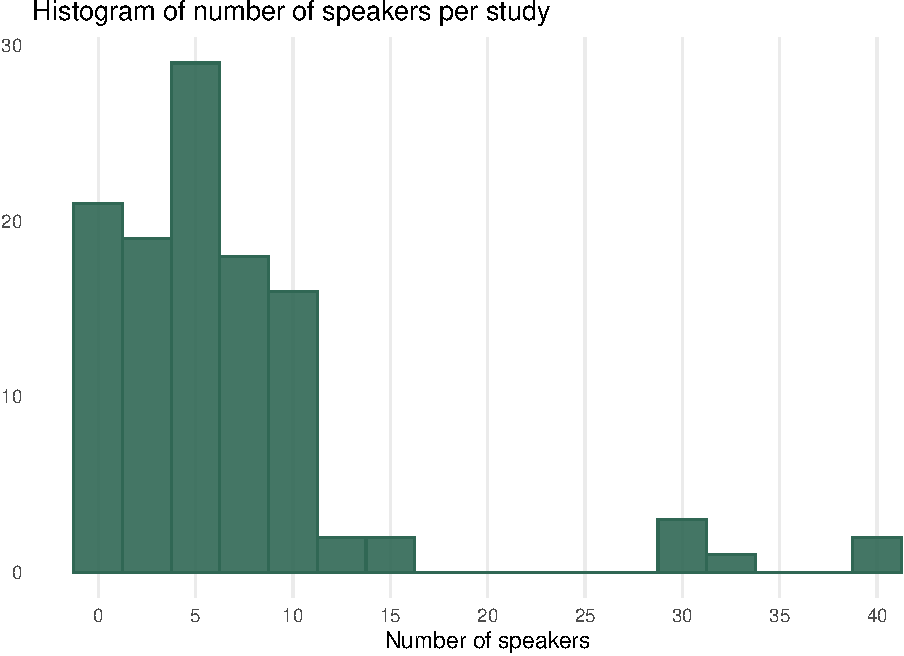
\includegraphics{2020-os_files/figure-latex/hist-1.pdf}

The following plot shows the number of speakers across publication year.
There is a tendecy for an increase in number of speakers, although the
trend is not particularly marked.

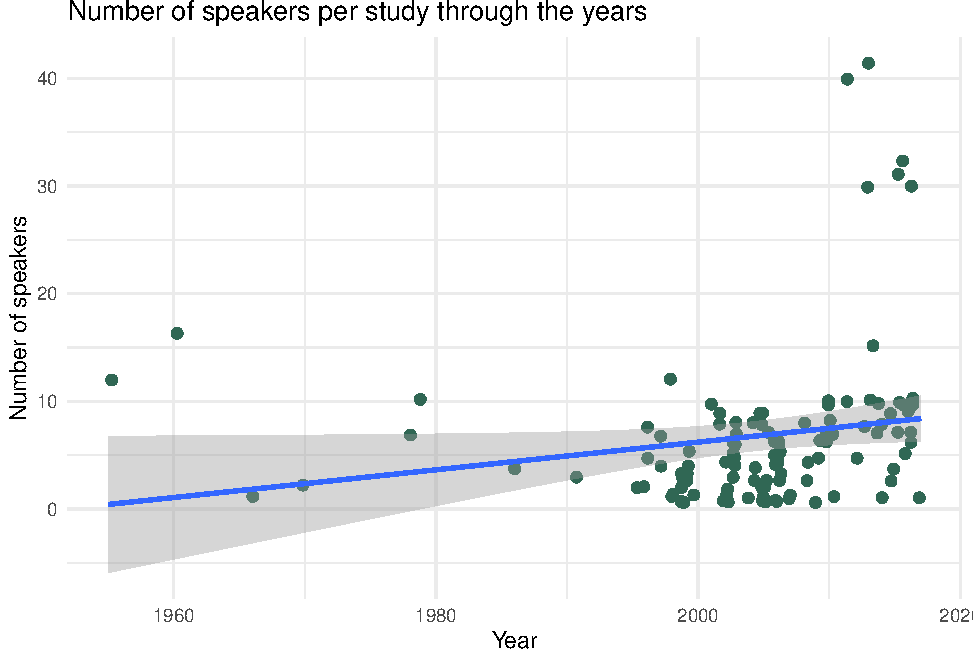
\includegraphics{2020-os_files/figure-latex/year-1.pdf}

The following bar chart shows the median number of speakers in studies
grouped by linguistic affiliation. The colour of the bars indicates the
number of studies. Indo-European languages stand out in terms of number
of studies (\textgreater{} 30), but the median number of speakers in
this family does not fare much better than other less-reachable
families.

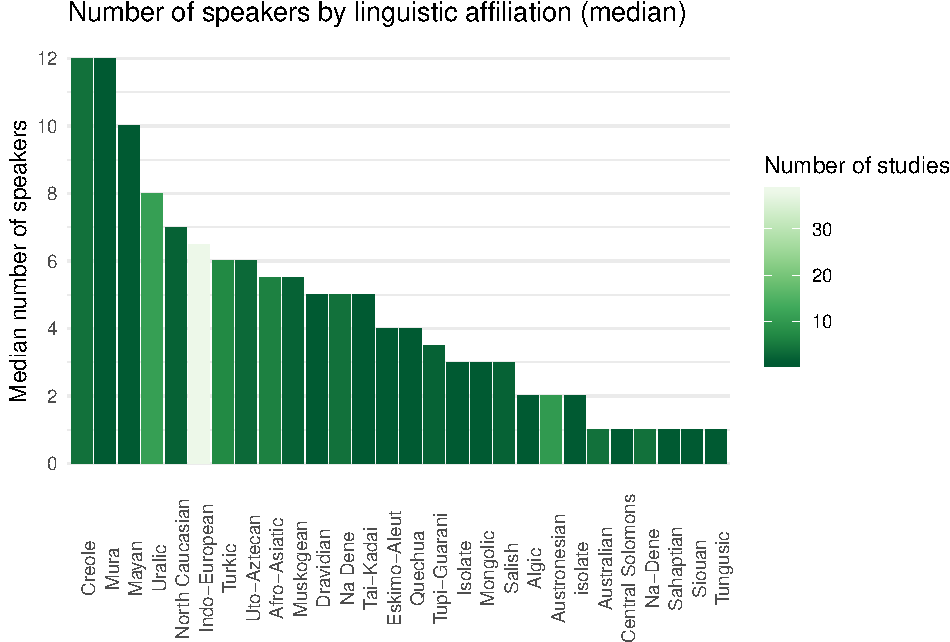
\includegraphics{2020-os_files/figure-latex/participants-affiliation-1.pdf}

Information on the endangerment status of the languages in the dataset
was obtained from
GlottoLog.\footnote{\url{https://glottolog.org/meta/downloads}.} The
following strip chart shows the number of speakers for each of the
studies (each point) categorised by the endangerment of the target
language. With the caveat that there are more studies on safe languages,
there is a trend of decreasing number of speakers from safe, to
vulnerable, to definitely endangered languages. The very low number of
studies on languages of greater endangerment status makes it harder to
establish patterns. Note also that the decreasing trend is in fact small
(1/2 speakers).

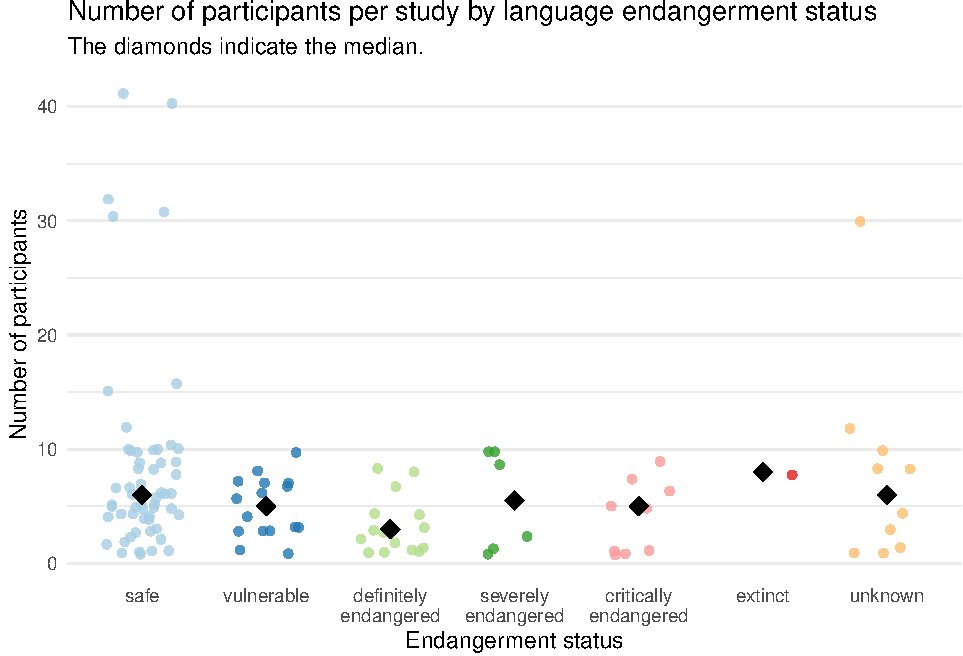
\includegraphics{2020-os_files/figure-latex/status-1.pdf}

While generalisations based on this cursory analysis would not be wise,
there seems to be a tendency for studies to have a very low number of
speakers (median 5 speakers per study). The majority of studies analysed
data from 10 speakers or less. This estimate is independent of
publication year and endangerment status of the language enquired.

\bibliography{linguistics}

\end{document}
